El modelo de datos es el siguiente: \\
\begin{figure}[H]
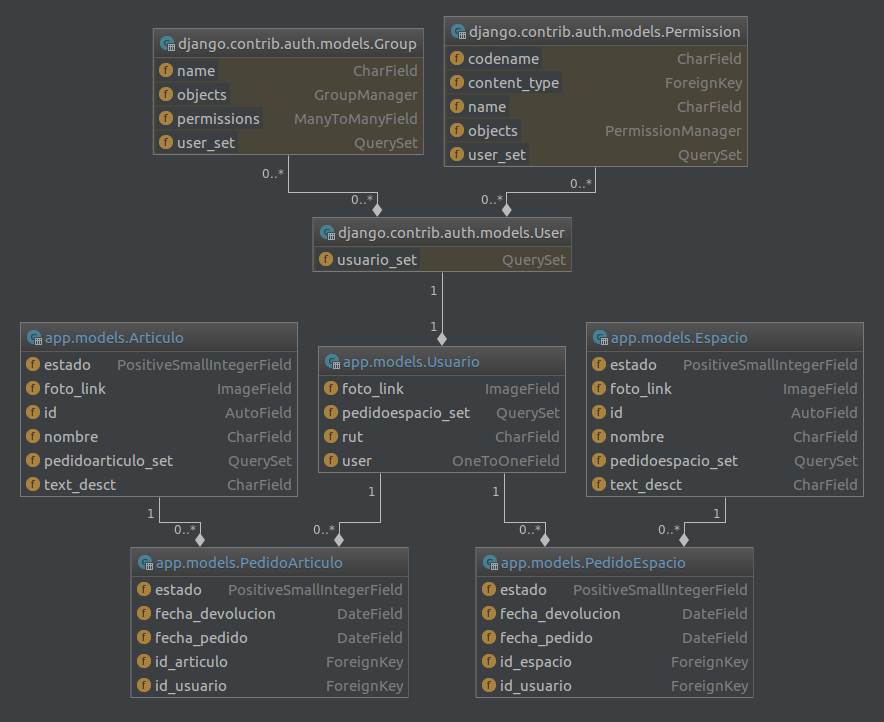
\includegraphics[width=0.5\textheight]{images/modelo_de_datos.png}
\caption{Diagrama del modelo de datos implementado} \label{LPUser}
\end{figure}
En este modelo se pueden distinguir tres niveles: un primer nivel generado automaticamente por Django en cuanto se utilizan sus modelos de Groups, Permission y User; un segundo nivel creado por el equipo donde se encuentran los elementos directamente relacionados con los requisitos que son los Artículos, Usuarios y Espacios; el último nivel es creado también por el equipo, pero son tablas relacionales entre los usuarios y artículos y espacios que representan los pedidos realizados por los usuarios y los resultados históricos de estas solicitudes.
Los modelos del primer nivel permiten generar un sistema de creación de usuario y logín con facilidad. Estos modelos disponen de nombre, apellido, correo, clave, permisos y grupos, todo ello por defecto dentro de Django. Así, podemos diferenciar una Persona Natural de un Administrador utilizando grupos, dando permisos por separado a cada grupo según lo indicado en los requisitos, así como poder guardar la información requerida por los usuarios. \\
Sin embargo, se hace necesario complementar esta información con datos adicionales que no corresponden al modelo de Django. Para ello, en el segundo nivel del modelo se extiende el usuario por defecto de Django con un usuario personalizado con nueva información adicional, como el rut y la foto de perfil; esta información servira para poblar de contenido el perfil del usuario. Además, consideramos tablas adicionales para los artículos y los espacios que dispondra el sistema para prestar a sus usuarios. La información que ahí se almacena servira para poder poblar las fichas de los artículos y espacios. \\
El último nivel, que posee las tablas relacionales entre usuario y artículo, y usuario y espacio; estas tablas almacenan la información de los pedidos hechos por un usuario, la fecha de pedido y devolución. Esta información se puede usar por el perfil del usuario como un registro histórico de sus pedidos, además de poder indicar al sistema que elementos se encuentran disponibles para que otros usuarios puedan pedir o no un artículo (según las fechas de los pedidos), así como informar a los administradores sobre la vigencia o caducidad de una solicitud (entre otros posibles). 